\documentclass{article}

\usepackage{amssymb,amsmath,amsthm, tikz}

\title{Assignment 6}
\author{Grace Garmire}
\date{}

\setlength{\parindent}{0eM}

\setlength{\parskip}{1.5ex plus 1ex minus 1ex}

\begin{document}

\maketitle
\thispagestyle{empty}

\textbf{Task 1:} Draw the graph of the function $\sqrt{x}$ on the interval $[0,4]$.

\begin{center}
  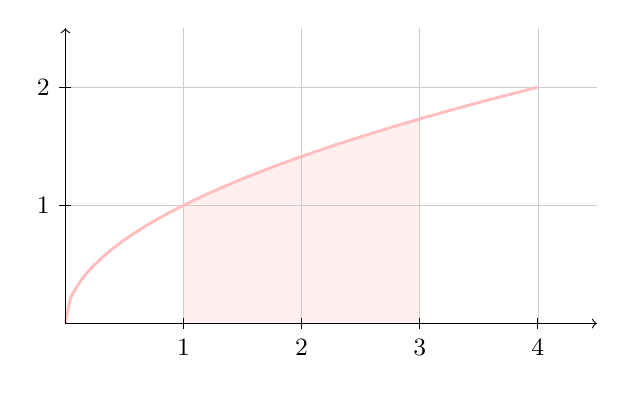
\begin{tikzpicture}[scale = 1.5]
    \draw [black!20, very thin] (0,0) grid (4.5,2.5);
    \fill [domain=1:3,
    smooth,
    pink,
    opacity = .25,
    samples = 100]
    (1,0) -- plot (\x, {pow(\x, .5)}) -- (3,0) -- cycle;
    \draw [domain=0:4,
    smooth,
    line width = .25ex,
    pink,
    samples = 100]
    plot (\x, {pow(\x, .5)});
    \draw [->, thin] (0,0) -- (0,2.5);
    \draw [->, thin] (0,0) -- (4.5,0);
    \foreach \x in {1,2,3,4} {
      \draw (\x, .05) -- (\x, -.05) node [below]
      {\begin{small}$\x$\end{small}};
    }
    \foreach \x in {1,2} {
      \draw (.05, \x) -- (-.05, \x) node [left]
      {\begin{small}$\x$\end{small}};
    }
  \end{tikzpicture}
\end{center}

\textbf{Task 2:} Draw at least one of the five representations of the Wagner graph.

One representation:
\begin{center}
  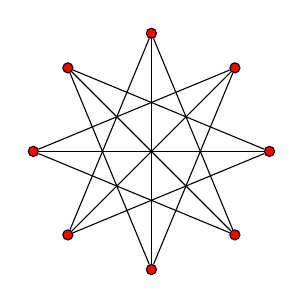
\begin{tikzpicture}[scale = 1.5]
    \tikzstyle{every node} = [draw, circle, fill = red!100, inner sep = .3ex];
    % points:
    \node (v0) at (1,0){};
    \node (v1) at (0.7071,0.7071){};
    \node (v2) at (0,1){};
    \node (v3) at (-0.7071,0.7071){};
    \node (v4) at (-1,0){};
    \node (v5) at (-0.7071,-0.7071){};
    \node (v6) at (0,-1){};
    \node (v7) at (0.7071,-0.7071){};
    % lines:
    \draw (v0) -- (v3); \draw (v0) -- (v4); \draw (v0) -- (v5);
    \draw (v1) -- (v4); \draw (v1) -- (v5); \draw (v1) -- (v6);
    \draw (v2) -- (v5); \draw (v2) -- (v6); \draw (v2) -- (v7);
    \draw (v3) -- (v6); \draw (v3) -- (v7);
    \draw (v4) -- (v7);
  \end{tikzpicture}
\end{center}

Another representation:
\begin{center}
  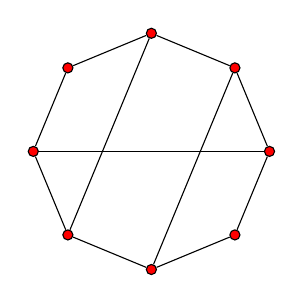
\begin{tikzpicture}[scale = 1.5]
    \tikzstyle{every node} = [draw, circle, fill = red!100, inner sep = .3ex];
    % points:
    \node (v0) at (1,0){};
    \node (v1) at (0.7071,0.7071){};
    \node (v2) at (0,1){};
    \node (v3) at (-0.7071,0.7071){};
    \node (v4) at (-1,0){};
    \node (v5) at (-0.7071,-0.7071){};
    \node (v6) at (0,-1){};
    \node (v7) at (0.7071,-0.7071){};
    % lines:
    \draw (v0) -- (v1) --  (v2) -- (v3) -- (v4) -- (v5) -- (v6) -- (v7) -- (v0);
    \draw (v1) -- (v6); \draw (v2) -- (v5);
    \draw (v0) -- (v4);
  \end{tikzpicture}
\end{center}

One more representation:
\begin{center}
  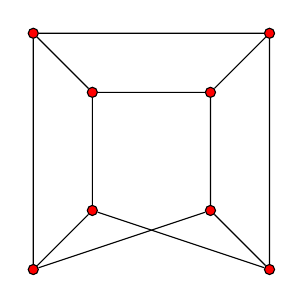
\begin{tikzpicture}[scale = .75]
    \tikzstyle{every node} = [draw, circle, fill = red!100, inner sep = .3ex];
    % points:
    \node (s0) at (0,0){};
    \node (s1) at (4,0){};
    \node (s2) at (4,4){};
    \node (s3) at (0,4){};
    \node (s4) at (1,1){};
    \node (s5) at (3,1){};
    \node (s6) at (3,3){};
    \node (s7) at (1,3){};
    \draw (s1) -- (s2) -- (s3) -- (s0) -- (s4) -- (s7) -- (s6) -- (s5) -- (s1);
    \draw (s0) -- (s5); \draw (s1) -- (s4);
    \draw (s2) -- (s6); \draw (s3) -- (s7);
  \end{tikzpicture}
\end{center}

\end{document}